% ============================================================================
% Lean4-Automata — LaTeX Architecture Anchor
% Compilable with: pdflatex LATEX_ANCHOR.tex
% ============================================================================
\documentclass[11pt,a4paper]{article}

% ── Packages ────────────────────────────────────────────────────────────────
\usepackage[utf8]{inputenc}
\usepackage[T1]{fontenc}
\usepackage{lmodern}
\usepackage[margin=2.5cm]{geometry}
\usepackage{hyperref}
\usepackage{xcolor}
\usepackage{listings}
\usepackage{booktabs}
\usepackage{longtable}
\usepackage{tikz}
\usepackage{enumitem}
\usepackage{fancyhdr}
\usepackage{titlesec}

\usetikzlibrary{shapes.geometric, arrows.meta, positioning, fit, backgrounds}

% ── Colors ──────────────────────────────────────────────────────────────────
\definecolor{codeblue}{HTML}{268BD2}
\definecolor{codegreen}{HTML}{859900}
\definecolor{codegray}{HTML}{93A1A1}
\definecolor{codebg}{HTML}{FDF6E3}
\definecolor{svcblue}{HTML}{4A90D9}
\definecolor{svcgreen}{HTML}{50C878}
\definecolor{svcred}{HTML}{E74C3C}
\definecolor{svcgold}{HTML}{F39C12}

% ── Listings Style ──────────────────────────────────────────────────────────
\lstset{
  backgroundcolor=\color{codebg},
  basicstyle=\ttfamily\small,
  breakatwhitespace=false,
  breaklines=true,
  captionpos=b,
  commentstyle=\color{codegreen},
  keywordstyle=\color{codeblue}\bfseries,
  stringstyle=\color{svcred},
  numberstyle=\tiny\color{codegray},
  numbers=left,
  numbersep=8pt,
  frame=single,
  rulecolor=\color{codegray},
  tabsize=4,
  showstringspaces=false,
}

\lstdefinelanguage{SQL}{
  morekeywords={SELECT,FROM,WHERE,JOIN,ON,ORDER,BY,LIMIT,INSERT,INTO,
    VALUES,UPDATE,SET,DELETE,CREATE,TABLE,VIEW,INDEX,WITH,RECURSIVE,
    UNION,AS,AND,OR,NOT,NULL,TRUE,FALSE,ASC,DESC,MATERIALIZED,
    CONCURRENTLY,REFRESH,USING,GIN,COALESCE,CASE,WHEN,THEN,ELSE,END},
  sensitive=false,
  morestring=[b]',
  morecomment=[l]{--},
}

% ── Headers ─────────────────────────────────────────────────────────────────
\pagestyle{fancy}
\fancyhf{}
\fancyhead[L]{\textsc{Lean4-Automata}}
\fancyhead[R]{\textsc{Architecture Reference}}
\fancyfoot[C]{\thepage}

% ── Title ───────────────────────────────────────────────────────────────────
\title{%
  \textbf{Lean4-Automata} \\[0.3em]
  \Large Architecture \& Technical Reference
}
\author{Generated from codebase analysis}
\date{\today}

% ============================================================================
\begin{document}
\maketitle
\tableofcontents
\newpage

% ============================================================================
\section{System Overview}
% ============================================================================

Lean4-Automata is a full-stack code-intelligence platform for the Lean~4
theorem prover. It parses \texttt{.lean} source files, extracts symbols
(theorems, definitions, instances, etc.), tracks inter-symbol dependencies,
computes static-analysis metrics, and serves the results through RESTful
APIs, Server-Sent Events, and a Go-powered forum harness.

\subsection{Design Goals}
\begin{enumerate}[label=(\roman*)]
  \item \textbf{Incremental indexing} --- detect file changes via inotify and
        re-index only modified files.
  \item \textbf{Rich static analysis} --- proof completion (\texttt{sorry}/\texttt{admit}
        tracking), floating-symbol detection, dependency centrality.
  \item \textbf{Real-time invalidation} --- SSE stream notifies clients when
        indexed data changes.
  \item \textbf{Secure by default} --- JWT auth on admin endpoints, compile-time
        flow registry, rate limiting, XSS protections.
  \item \textbf{Observable} --- optional Grafana + Loki stack, Flower for
        Celery monitoring, structured health endpoints.
\end{enumerate}

% ============================================================================
\section{Architecture Diagram}
% ============================================================================

\begin{figure}[ht]
\centering
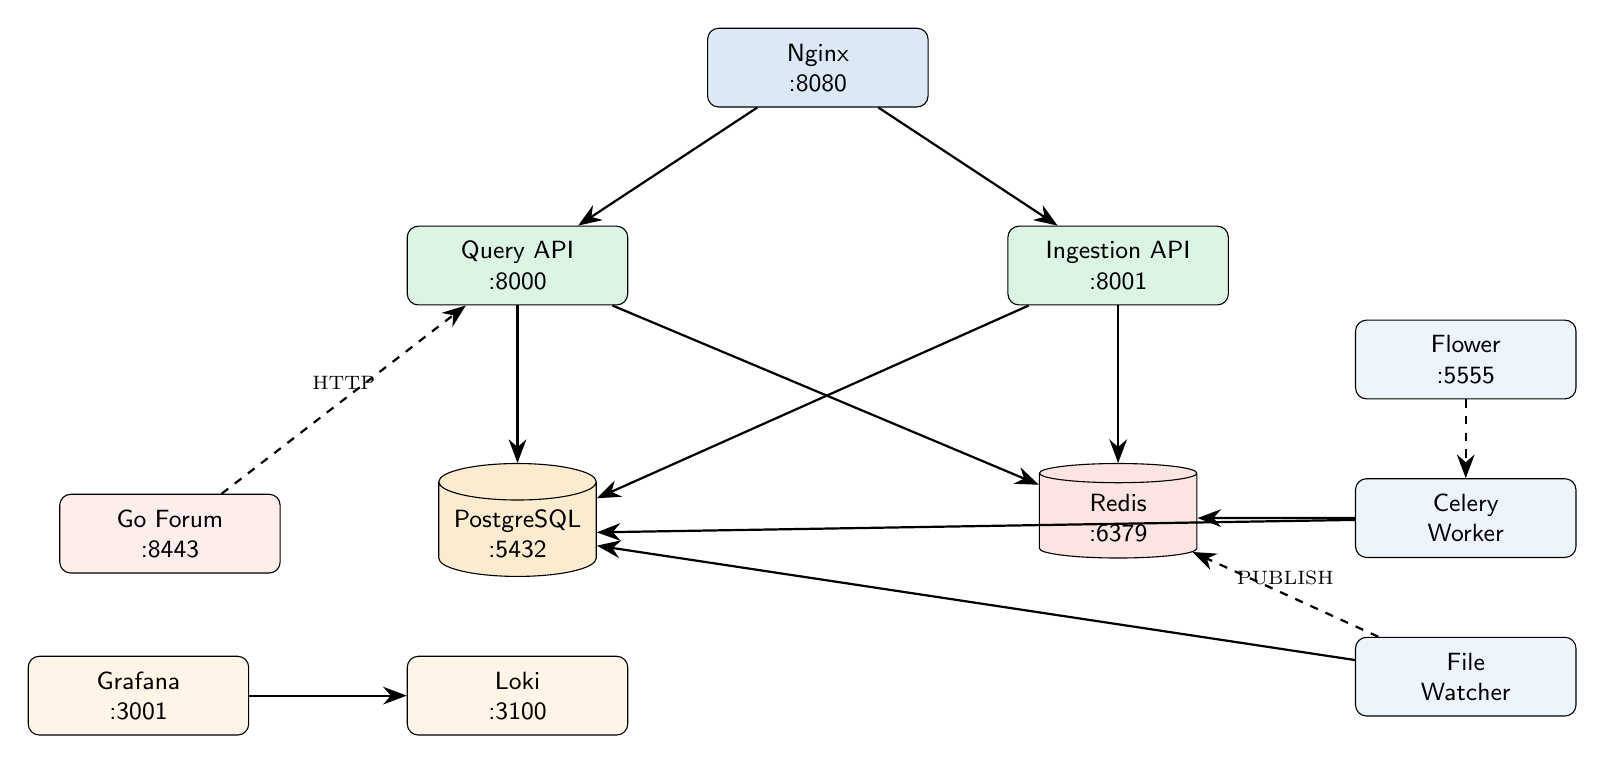
\begin{tikzpicture}[
  node distance=1.5cm and 2.0cm,
  svc/.style={rectangle, draw, rounded corners, minimum width=2.8cm,
              minimum height=1cm, font=\small\sffamily, align=center},
  db/.style={cylinder, draw, shape border rotate=90, aspect=0.25,
             minimum width=2cm, minimum height=1.2cm,
             font=\small\sffamily, align=center},
  arr/.style={-{Stealth[length=3mm]}, thick},
  darr/.style={-{Stealth[length=3mm]}, thick, dashed},
]

% -- Nginx
\node[svc, fill=svcblue!20] (nginx) {Nginx\\:8080};

% -- APIs
\node[svc, fill=svcgreen!20, below left=1.5cm and 1cm of nginx] (query) {Query API\\:8000};
\node[svc, fill=svcgreen!20, below right=1.5cm and 1cm of nginx] (ingest) {Ingestion API\\:8001};

% -- Data stores
\node[db, fill=svcgold!20, below=2cm of query] (pg) {PostgreSQL\\:5432};
\node[db, fill=svcred!15, below=2cm of ingest] (redis) {Redis\\:6379};

% -- Workers
\node[svc, fill=svcblue!10, right=2cm of redis] (worker) {Celery\\Worker};
\node[svc, fill=svcblue!10, below=1cm of worker] (watcher) {File\\Watcher};
\node[svc, fill=svcblue!10, above=1cm of worker] (flower) {Flower\\:5555};

% -- Go Forum
\node[svc, fill=svcred!10, left=2cm of pg] (forum) {Go Forum\\:8443};

% -- Observability
\node[svc, fill=svcgold!10, below=1cm of pg] (loki) {Loki\\:3100};
\node[svc, fill=svcgold!10, left=2cm of loki] (grafana) {Grafana\\:3001};

% -- Arrows
\draw[arr] (nginx) -- (query);
\draw[arr] (nginx) -- (ingest);
\draw[arr] (query) -- (pg);
\draw[arr] (query) -- (redis);
\draw[arr] (ingest) -- (redis);
\draw[arr] (ingest) -- (pg);
\draw[arr] (worker) -- (pg);
\draw[arr] (worker) -- (redis);
\draw[arr] (watcher) -- (pg);
\draw[darr] (watcher) -- (redis) node[midway, above, font=\scriptsize] {PUBLISH};
\draw[darr] (forum) -- (query) node[midway, above, font=\scriptsize] {HTTP};
\draw[arr] (grafana) -- (loki);
\draw[darr] (flower) -- (worker);

\end{tikzpicture}
\caption{High-level service topology. Dashed arrows indicate async or pub/sub communication.}
\label{fig:arch}
\end{figure}

% ============================================================================
\section{Service Directory}
% ============================================================================

\begin{longtable}{@{}lllp{5.5cm}@{}}
\toprule
\textbf{Service} & \textbf{Port} & \textbf{Image} & \textbf{Purpose} \\
\midrule
\endhead
postgres     & 5432 & postgres:17          & Primary data store \\
redis        & 6379 & redis:7              & Cache, Celery broker, pub/sub \\
nginx        & 8080 & nginx:stable         & Reverse proxy, rate limiting \\
app          & 8000 & Dockerfile.api       & Public query API (FastAPI) \\
app\_ingestion & 8001 & Dockerfile.ingestion & Admin ingestion API (FastAPI) \\
worker       & ---  & Dockerfile.worker    & Celery task workers \\
watcher      & ---  & Dockerfile.worker    & inotify file watcher daemon \\
flower       & 5555 & mher/flower:2.0      & Celery monitoring UI \\
web          & 3000 & frontend/Dockerfile  & Next.js frontend \\
loki         & 3100 & grafana/loki:3.4.2   & Log aggregation (optional) \\
grafana      & 3001 & grafana/grafana:11.6.0 & Dashboards (optional) \\
\bottomrule
\end{longtable}

% ============================================================================
\section{Data Model}
% ============================================================================

\subsection{PostgreSQL Tables}

The schema is managed by Alembic across four migrations:

\begin{enumerate}
  \item \textbf{0001}: Core tables --- \texttt{projects}, \texttt{files},
        \texttt{symbols}, \texttt{dependencies}, \texttt{file\_dependencies},
        \texttt{index\_runs}; enums \texttt{symbol\_kind}, \texttt{dependency\_type}.
  \item \textbf{0002}: Indexes --- B-tree on FK/filter columns, GIN on JSONB
        (\texttt{imports}, \texttt{attributes}), GIN full-text search on
        \texttt{symbols}.
  \item \textbf{0003}: Materialized views --- \texttt{dependency\_stats},
        \texttt{module\_metrics} (refreshed hourly by Celery beat).
  \item \textbf{0004}: Enriched file metrics (15+ columns), \texttt{has\_sorry}
        on symbols, SQL views \texttt{v\_proof\_status},
        \texttt{v\_floating\_symbols}, \texttt{v\_file\_interconnect}.
\end{enumerate}

\subsection{Symbol Kinds}

\begin{tabular}{@{}ll@{}}
\toprule
\textbf{Enum Value} & \textbf{Lean~4 Declaration} \\
\midrule
theorem   & \texttt{theorem}, \texttt{lemma} \\
def       & \texttt{def} \\
axiom     & \texttt{axiom} \\
instance  & \texttt{instance} \\
inductive & \texttt{inductive} \\
structure & \texttt{structure} \\
class     & \texttt{class} \\
constant  & (reserved) \\
opaque    & \texttt{opaque} \\
abbrev    & \texttt{abbrev} \\
\bottomrule
\end{tabular}

\subsection{Key Views}

\begin{tabular}{@{}lp{9cm}@{}}
\toprule
\textbf{View} & \textbf{Purpose} \\
\midrule
\texttt{v\_proof\_status}      & Per-file proof completeness with status labels
                                 (complete, partial, mostly\_incomplete, no\_theorems) \\
\texttt{v\_floating\_symbols}  & Public theorems/defs with zero incoming cross-file
                                 dependencies --- ``proved but never used'' \\
\texttt{v\_file\_interconnect} & File-level fan-in/fan-out, Mathlib vs.\ local imports \\
\texttt{dependency\_stats}     & Per-symbol fan-in, fan-out, total connections (MV) \\
\texttt{module\_metrics}       & Per-module symbol counts, doc coverage (MV) \\
\bottomrule
\end{tabular}

% ============================================================================
\section{API Reference}
% ============================================================================

\subsection{Query API (:8000)}

\begin{longtable}{@{}llp{7.5cm}@{}}
\toprule
\textbf{Method} & \textbf{Path} & \textbf{Description} \\
\midrule
\endhead
GET & \texttt{/health/live}                    & Liveness probe \\
GET & \texttt{/health/ready}                   & Readiness (DB + Redis check) \\
GET & \texttt{/api/v1/symbols/search}          & Full-text search (\texttt{q}, \texttt{project\_id},
                                                  \texttt{limit}, \texttt{offset}) \\
GET & \texttt{/api/v1/symbols/\{full\_name\}}  & Symbol lookup by qualified name \\
GET & \texttt{/api/v1/dependencies/graph}       & Transitive + reverse dependency graph \\
GET & \texttt{/api/v1/modules/metrics}          & Module-level aggregated metrics \\
GET & \texttt{/api/v1/events/invalidation}      & SSE cache-invalidation stream \\
\bottomrule
\end{longtable}

\subsection{Ingestion API (:8001, JWT-protected)}

\begin{longtable}{@{}llp{7.5cm}@{}}
\toprule
\textbf{Method} & \textbf{Path} & \textbf{Description} \\
\midrule
\endhead
POST & \texttt{/admin/index/start}              & Enqueue full-scan Celery task \\
GET  & \texttt{/admin/index/status/\{task\_id\}} & Poll task state \\
\bottomrule
\end{longtable}

% ============================================================================
\section{Parser Architecture}
% ============================================================================

The Lean~4 parser (\texttt{parser/lean\_parser.py}) is regex-based and
operates in four stages:

\begin{enumerate}
  \item \textbf{Comment/string stripping} --- length-preserving replacement
        with spaces to maintain accurate line numbers.
  \item \textbf{Namespace tracking} --- stack-based, tracking
        \texttt{namespace Foo} blocks and their indentation levels.
  \item \textbf{Declaration scanning} --- regex matching against 11 declaration
        kinds (\texttt{def}, \texttt{theorem}, \texttt{lemma}, \texttt{instance},
        \texttt{class}, \texttt{structure}, \texttt{inductive}, \texttt{abbrev},
        \texttt{axiom}, \texttt{example}, \texttt{opaque}).
  \item \textbf{Metric computation} --- regex scans for \texttt{sorry},
        \texttt{admit}, \texttt{native\_decide}, debug commands, etc.
\end{enumerate}

Each parsed symbol produces a \texttt{ParsedSymbol} dataclass:

\begin{lstlisting}[language=Python, caption={ParsedSymbol dataclass}]
@dataclass
class ParsedSymbol:
    name: str
    kind: str               # "theorem", "def", etc.
    line_start: int
    namespace_path: list[str]
    is_private: bool
    signature_text: str
    mods: list[str]         # ["noncomputable", "protected"]
    has_sorry: bool
\end{lstlisting}

% ============================================================================
\section{Security Model}
% ============================================================================

\begin{longtable}{@{}lp{4cm}p{6.5cm}@{}}
\toprule
\textbf{Layer} & \textbf{Mechanism} & \textbf{Detail} \\
\midrule
\endhead
Auth          & JWT Bearer (HS256)        & Admin role required for ingestion API;
                                            Swagger/Redoc disabled in production \\
CORS          & Strict origin list        & Query API: GET+OPTIONS only;
                                            configurable via \texttt{ALLOWED\_ORIGINS} \\
Rate limit    & Nginx \texttt{limit\_req} & 60 req/min on search, burst=20;
                                            10 SSE connections per IP \\
Input valid.  & Request-ID regex          & \texttt{\^{}[a-zA-Z0-9-]\{1,64\}\$} --- log injection
                                            prevention \\
Code exec     & Compile-time registry     & Go FlowFunc map --- no DB-driven command
                                            templates (commit \texttt{10927ba}) \\
XSS           & Output encoding           & JSON.stringify in SSE output;
                                            \texttt{textContent} for user text in UI \\
Body size     & 1\,MB limit               & Go forum enforces max request body \\
Server info   & \texttt{server\_tokens off} & Nginx hides version string \\
\bottomrule
\end{longtable}

% ============================================================================
\section{Observability}
% ============================================================================

\subsection{Log Aggregation}

All container logs are shipped to Loki via the Docker Loki logging driver.
Labels are attached per service name, enabling queries like:

\begin{lstlisting}[language=bash, caption={LogQL examples}]
{service="app"} |= "ERROR"
{service="worker"} |= "Task lean4.full_scan" |= "succeeded"
{service="nginx"} | json | status >= 500
\end{lstlisting}

\subsection{Dashboards}

Grafana is provisioned at port 3001 with Loki as the default data source.
Recommended dashboard panels:

\begin{itemize}
  \item \textbf{API Health}: time-series of \texttt{/health/ready} response codes
  \item \textbf{Task Throughput}: Celery task completion rate from Flower API
  \item \textbf{Cache Efficiency}: Redis hit/miss ratio
  \item \textbf{Rate Limiting}: count of 429 responses from Nginx
  \item \textbf{Proof Coverage}: aggregate \texttt{proof\_completion} from
        \texttt{v\_proof\_status}
\end{itemize}

% ============================================================================
\section{Deployment}
% ============================================================================

\subsection{Quick Start}

\begin{lstlisting}[language=bash, caption={Core stack startup}]
# Copy and edit environment
cp .env.example .env

# Start core services
docker compose up -d

# Run migrations
docker compose exec app alembic upgrade head

# Verify health
curl http://localhost:8000/health/ready
\end{lstlisting}

\subsection{With Observability}

\begin{lstlisting}[language=bash, caption={Full stack with observability}]
docker compose --profile observability up -d
# Grafana: http://localhost:3001 (admin/admin)
# Loki:    http://localhost:3100
# Flower:  http://localhost:5555
\end{lstlisting}

\subsection{Triggering a Full Index}

\begin{lstlisting}[language=bash, caption={Index a Lean project}]
curl -X POST http://localhost:8001/admin/index/start \
  -H "Authorization: Bearer $JWT" \
  -H "Content-Type: application/json" \
  -d '{"project_id": "1", "root_dir": "/lean-src"}'
\end{lstlisting}

% ============================================================================
\section{Environment Variables}
% ============================================================================

\begin{longtable}{@{}llp{6cm}@{}}
\toprule
\textbf{Variable} & \textbf{Default} & \textbf{Purpose} \\
\midrule
\endhead
APP\_PORT           & 8000                 & Query API port \\
INGESTION\_PORT     & 8001                 & Ingestion API port \\
NGINX\_HTTP\_PORT   & 8080                 & Nginx proxy port \\
POSTGRES\_DB        & lean4\_automata      & Database name \\
POSTGRES\_USER      & lean4                & Database user \\
REDIS\_URL          & redis://localhost:6379 & Redis connection string \\
DATABASE\_URL       & (asyncpg DSN)        & SQLAlchemy async DSN \\
JWT\_SECRET\_KEY    & CHANGE\_ME           & HMAC signing secret \\
JWT\_ALGORITHM      & HS256                & JWT algorithm \\
ENV                 & development          & Set \texttt{production} to disable docs \\
LEAN\_WATCH\_ROOT   & ./lean-src           & Watcher monitored directory \\
LEAN\_PROJECT\_ID   & 1                    & Default project ID \\
FLOW\_TIMEOUT\_SEC  & 30                   & Go forum per-flow timeout \\
MAX\_CONCURRENT\_FLOWS & 5                 & Go forum semaphore cap \\
\bottomrule
\end{longtable}

% ============================================================================
\section{Conclusion}
% ============================================================================

Lean4-Automata provides a comprehensive code-intelligence stack for Lean~4
projects, from low-level regex parsing to high-level proof-completion analytics.
The architecture separates concerns across FastAPI query/ingestion services,
Celery background workers, an inotify file watcher, and a Go forum harness,
with PostgreSQL for structured data and Redis for caching and real-time
event propagation. The optional Grafana+Loki observability stack and
Flower monitoring provide production-grade visibility into system health.

\end{document}
